\section{Implementation}\label{sec:03_impl}
% Explain section
This section explains the implementation based on the conceptual design introduced in \Sec{sec:02_design}.
% Which parts
Therefore, this applications is composed of two different parts: A backend, and a frontend.


\subsection{Backend}\label{subsec:03_impl_backend}
%
As introduced in \Sec{subsec:02_design_backend}, the backend part of the application is responsible for authentication, keeping a ranking list of games played by different users, and generating the grid for the Memory game.
% Servlets
To achieve this functionality, the following servlets are created:
\begin{itemize}
\item \textit{Welcome-Servlet}
\item \textit{Ranking-Servlet}
\item \textit{Memory-Play-Servlet}
\item \textit{Memory-Grid-Servlet}
\end{itemize}
% Filters
In addition to the servlets, a \textit{Welcome-Filter} needs to be implemented to check whenever a user is authenticated or not.

\subsubsection{Models}\label{subsubsec:03_impl_backend_models}
% What models
A user is allowed to authenticate itself with a username. Therefore, a model called \textit{User} is needed in the system.
% For what
This model will be used to authenticate the user on all pages, as introduced in \Sec{subsubsec:02_design_backend_auth}, and to save a ranking with all users who played a game before.

% Scoreboard
Additionally, the backend keeps track of a scoreboard to safe the points achieved by a user. This is achieved by the \textit{Scoreboard} model.
% How
The \textit{Scoreboard} model saves User models and their points in a Map object.
% Top 5
Additionally, the \textit{Scoreboard} model provides a method called \texttt{getTop5} that returns the Top 5 scores. This used for the \textit{Ranking-Page}.

% How
\Fig{fig:subsubsec:03_impl_backend_models_uml} describes both models. The \textit{User} model will be saved in the HTTP session of the client. However, the same scoreboard instance needs to be available for all users. Therefore, the \textit{Scoreboard} model is saved in the servlet-context.
% Java Bean
Additionally, to use these models in \texttt{JSP} views, both models follow the Java Bean specification.
% Model figure
\begin{figure}[h]
\centering
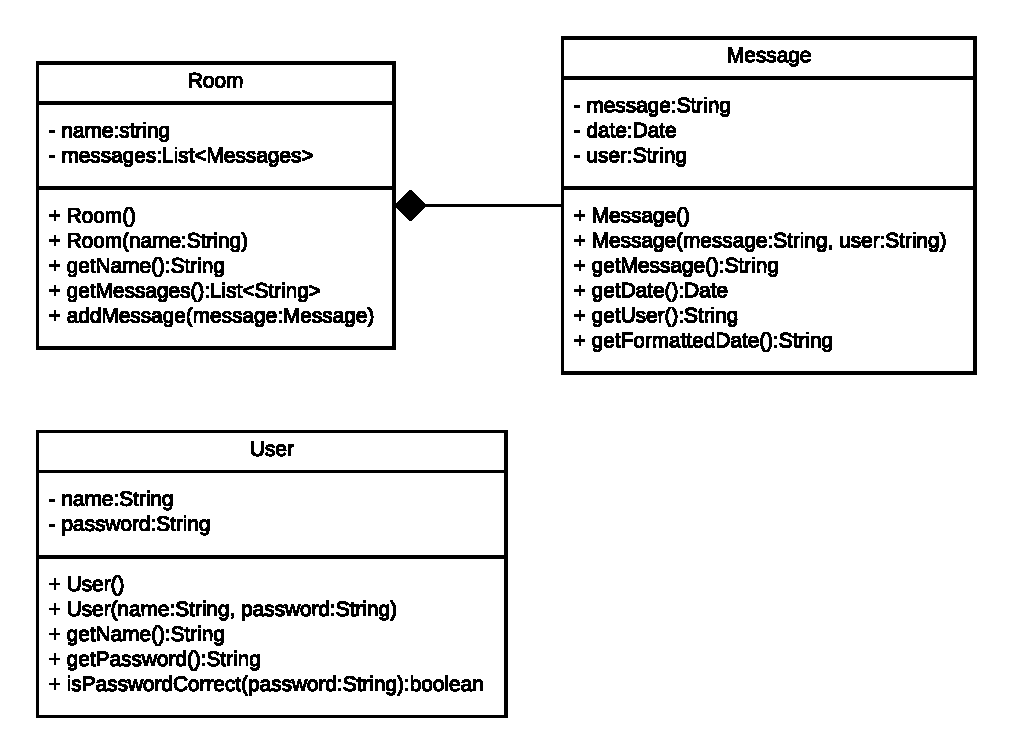
\includegraphics[scale=0.8]{images/03_impl/models}
\caption{UML diagram describing the models}
\label{fig:subsubsec:03_impl_backend_models_uml}
\end{figure}

\newpage
\subsubsection{Welcome}\label{subsubsec:03_impl_backend_welcome}
As introduced before, the user needs to authenticate itself with a username, and a password is not required. If the user is not authenticated, the user can not access the game or the ranking page.
% Where
A user can authenticate at the \textit{Welcome-Page}. There, the user user can enter a name in an \texttt{HTML} form, as illustrated in \Fig{fig:03_impl_backend_welcome_page}. After submitting the form, the username is being send as a \texttt{POST} request to the \textit{Welcome-Servlet}. After that, the \textit{Welcome-Servlet} validates the \texttt{POST} request. If the request is valid, a new \textit{User} model will be added to the client HTTP session. Then, the user will be forwarded to the \textit{Ranking-Page}.
% How
To ensure, that only authenticated users can access the \textit{Ranking-Page}, and the \textit{Memory-Play-Page}, a filter called Welcome-Filter is implemented, that checks if the a \textit{User} objects is available in the HTTP session of the client. If yes, the user is can access all pages, otherwise the user is being forwarded to the welcome page.
% Grid figure
\begin{figure}[h]
\centering
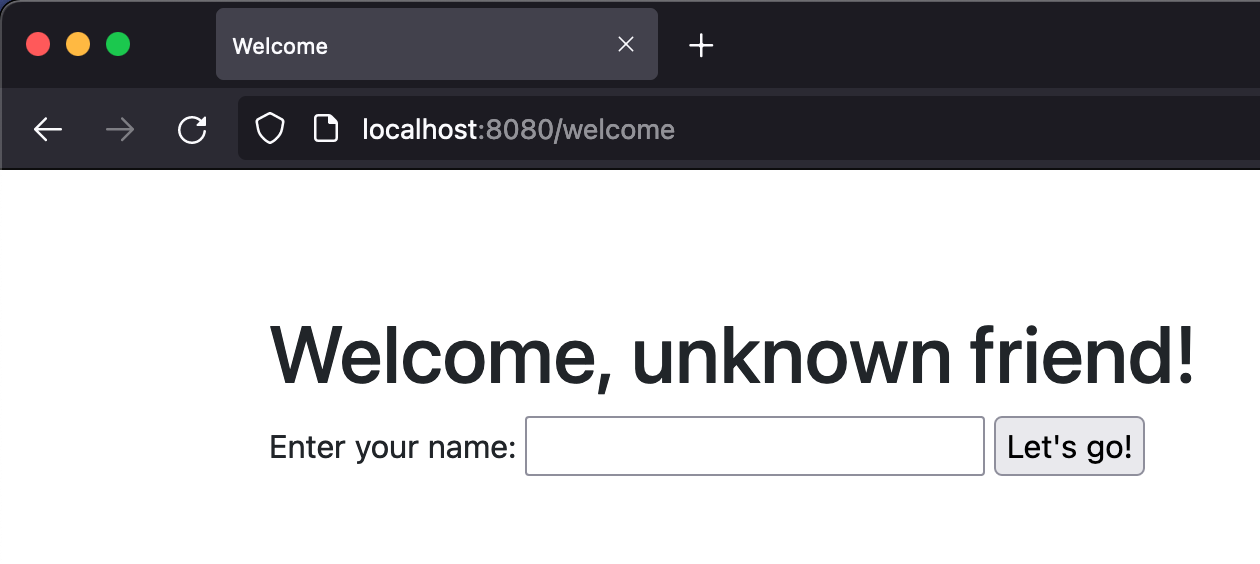
\includegraphics[scale=0.4]{images/03_impl/welcome/welcome-page}
\caption{The \textit{Welcome-Page}}
\label{fig:03_impl_backend_welcome_page}
\end{figure}

\subsubsection{Ranking}\label{subsubsec:03_impl_backend_ranking}
% What
The \textit{Ranking-Servlet} is responsible to keep track of all games played.

% Get request
If a \texttt{GET} request is send to the \textit{Ranking-Servlet}, it will response an \texttt{HTML} page with the ranking of the Top 5 users. The ranking displays the name and the points of the user. If no games have been played before, the ranking shows an empty list, as illustrated in \Fig{fig:03_impl_backend_ranking_page}.
% Grid figure
\begin{figure}[h]
\centering
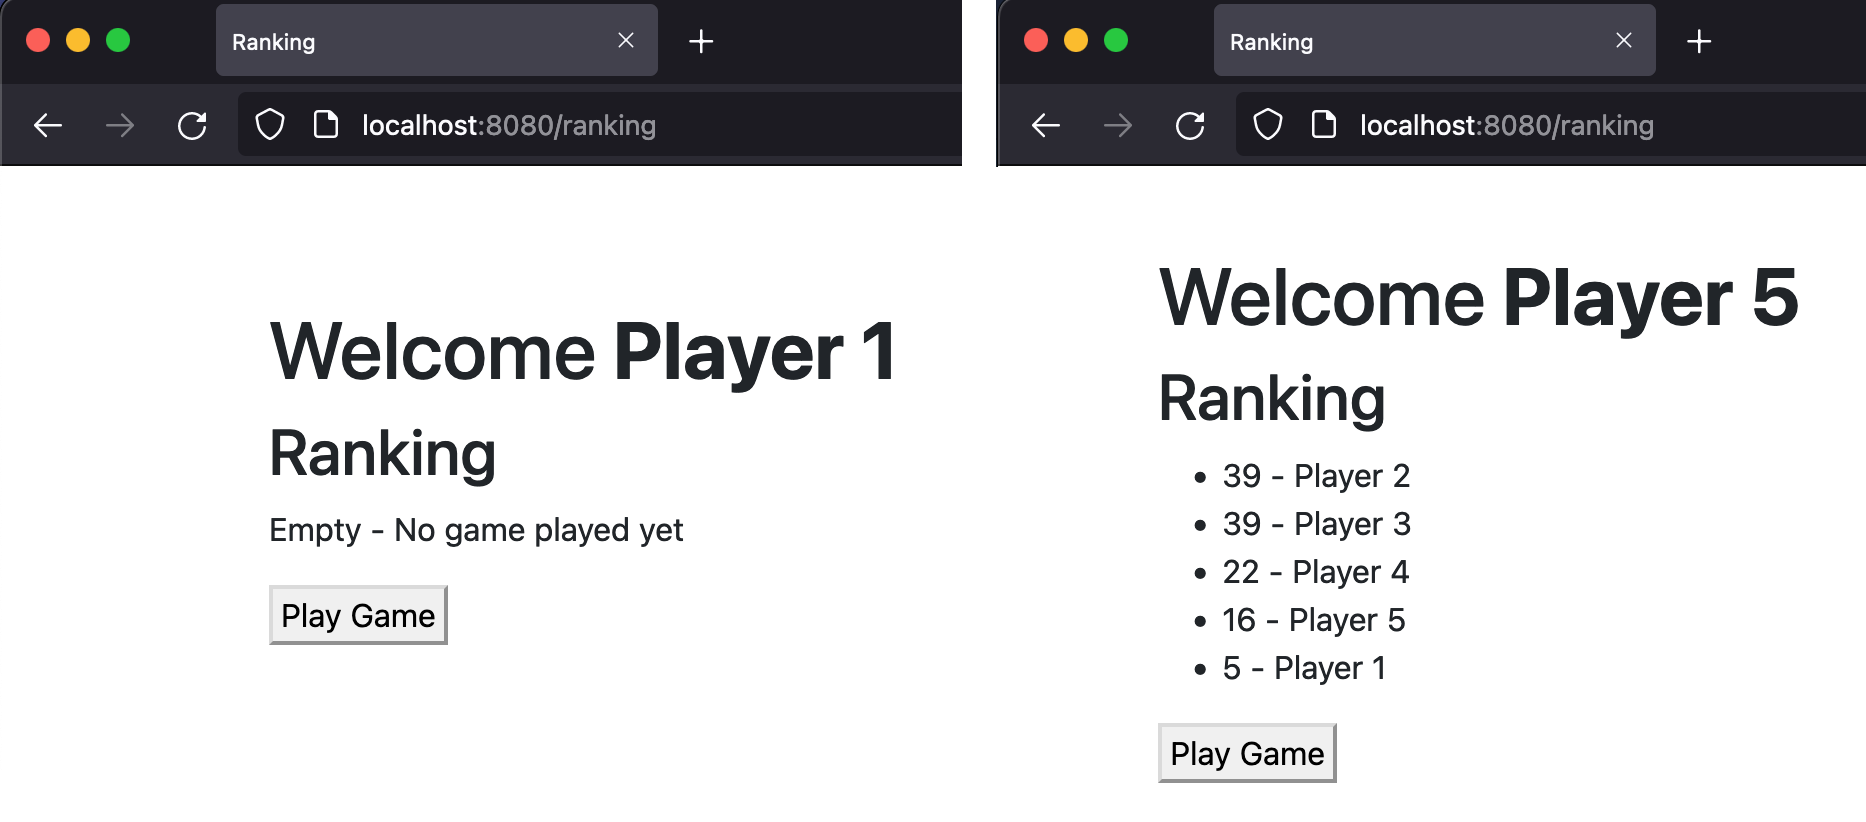
\includegraphics[scale=0.2]{images/03_impl/ranking/ranking}
\caption{The \textit{Ranking-Page} with an empty ranking on the left, and the Top 5 on the right}
\label{fig:03_impl_backend_ranking_page}
\end{figure}

% View
The view is implemented using a \texttt{JSP} view. It includes the current User and the Scoreboard via \texttt{jsp:useBean} to get its properties.
% SHow the Top5
Additionaly, it uses JSP - Standard Tag Library (JSTL) to show the Top 5 users, which is shown in \Lst{lst:03_impl_backend_ranking_jstl}. Furthermore, the ranking shows the name of the current user at the top.
% JSTL Listing
\begin{lstlisting}[label=lst:03_impl_backend_ranking_jstl, caption=Show the Top 5 using JSTL, language=html]
<%@ taglib prefix="c" uri="http://java.sun.com/jsp/jstl/core" %>
<jsp:useBean id="scoreboard" class="it.unitn.disi.webarch.memory.models.Scoreboard" scope="application"/>
<c:choose>
  <c:when test="${scoreboard.isEmpty()}">
    <p>Empty - No game played yet</p>
  </c:when>
  <c:otherwise>
    <ul>
      <c:forEach items="${scoreboard.getTop5()}" var="score">
        <li>${score.get(1)} - ${score.get(0).getName()}</li>
      </c:forEach>
    </ul>
  </c:otherwise>
</c:choose>
\end{lstlisting}


% POST request
To save a new score, the \textit{Ranking-Servlet} accepts \texttt{POST} request as well. It requires a number of points with the content-type of \texttt{application/x-www-form-urlencoded}.
% Save
The points will be added to the current score of the user of the client session using the \texttt{addScore} method of the \textit{Scoreboard} model.
% Where is it saved
The overall ranking needs to be available to all users. Therefore, it is saved in the servlet-context instead of the the HTTP session.
% Not persistant
It is important to mention, that it is not required to save the overall ranking persistently. Therefore, if the webserver exits, the servlet-context is removed from the host memory and wont be available after a restart. However, the ranking is available as long as the webserver is running.

\subsubsection{Grid}\label{subsubsec:03_impl_backend_grid}
% What
The \textit{Memory-Grid-Servlet} is reponsible to generate the grid for the memory game. The concept of the grid has been introduced in \Sec{subsubsec:02_design_backend_grid}.
% GET
To recieve the value of a index in the grid, the frontend has to send a \texttt{GET} request and attach the index value to the query string. For example, to get the value of the second card in the grid, the URL has to look like the \path{http://localhost/memory/grid?index=2}.
% Response
The \textit{Memory-Grid-Servlet} will response the card value of the given index in text/plain.

% Translate
As being mentioned, the grid is a 2D list, that contains multiple lists of integers. Each Integer represents the card value at the given index. Therefore, to get the value for the given index in the \texttt{GET} request, it has to be translated into a 2D index (index in column and index in row). \Lst{lst:03_impl_backend_backend_grid_translate} shows the method \texttt{translateIndexToValue} that is used to translate a single index into a 2D index which can be used to get the card value from the grid.
% Listing
\begin{lstlisting}[label=lst:03_impl_backend_backend_grid_translate, caption=The \texttt{translateIndexToValue} method, language=java]
Integer translateIndexToValue(int index) {
  int differentCards = 8;
  int colIndex = (int) Math.floor(index / (differentCards / 2));
  int rowIndex = index % (differentCards / 2);
  int selectedValue = this.grid.get(colIndex).get(rowIndex);
  return selectedValue;
}
\end{lstlisting}

% Modes
In addition, it is possible to set the operation mode, which decides if the grid is generated randomly or deterministic. This property is set as a \texttt{init-param} in the \path{web.xml}, as illustrated by \Lst{lst:03_impl_backend_backend_grid_mode}. Then, the \textit{Memory-Grid-Servlet} can read this value using \texttt{getInitParameter("mode")}.
% Listing
\begin{lstlisting}[label=lst:03_impl_backend_backend_grid_mode, caption=\texttt{init-param} to set the mode, language=xml]
<servlet>
  <servlet-name>MemoryGridServlet</servlet-name>
  <servlet-class>it.unitn.disi.webarch.memory.controller.memory.MemoryGridServlet</servlet-class>
  <init-param>
    <param-name>mode</param-name>
    <param-value>development</param-value>
  </init-param>
</servlet>
\end{lstlisting}


\newpage
\subsection{Frontend}\label{subsec:03_impl_frontend}
% What
The frontend part of this application is the User Interface (UI) for the memory game. It is complety written in JavaScript and HTML.
%
It is composed of the following parts:
\begin{itemize}
\item \path{index.html}
\item \path{game.js}
\item \path{memoryGame.js}
\end{itemize}

\subsubsection{index.html}\label{subsubsec:03_impl_frontend_index}
% WHat
The \textit{index.html} file defines the UI of the game, illustrated in \Fig{fig:03_impl_frontend_index_grid}. It shows the grid of memory cards, a label that shows the number of tries, and a label that shows the current points. Additionally, at the top there is a Game Over! that is shown after the user has finishes the game.
% Grid figure
\begin{figure}[h]
\centering
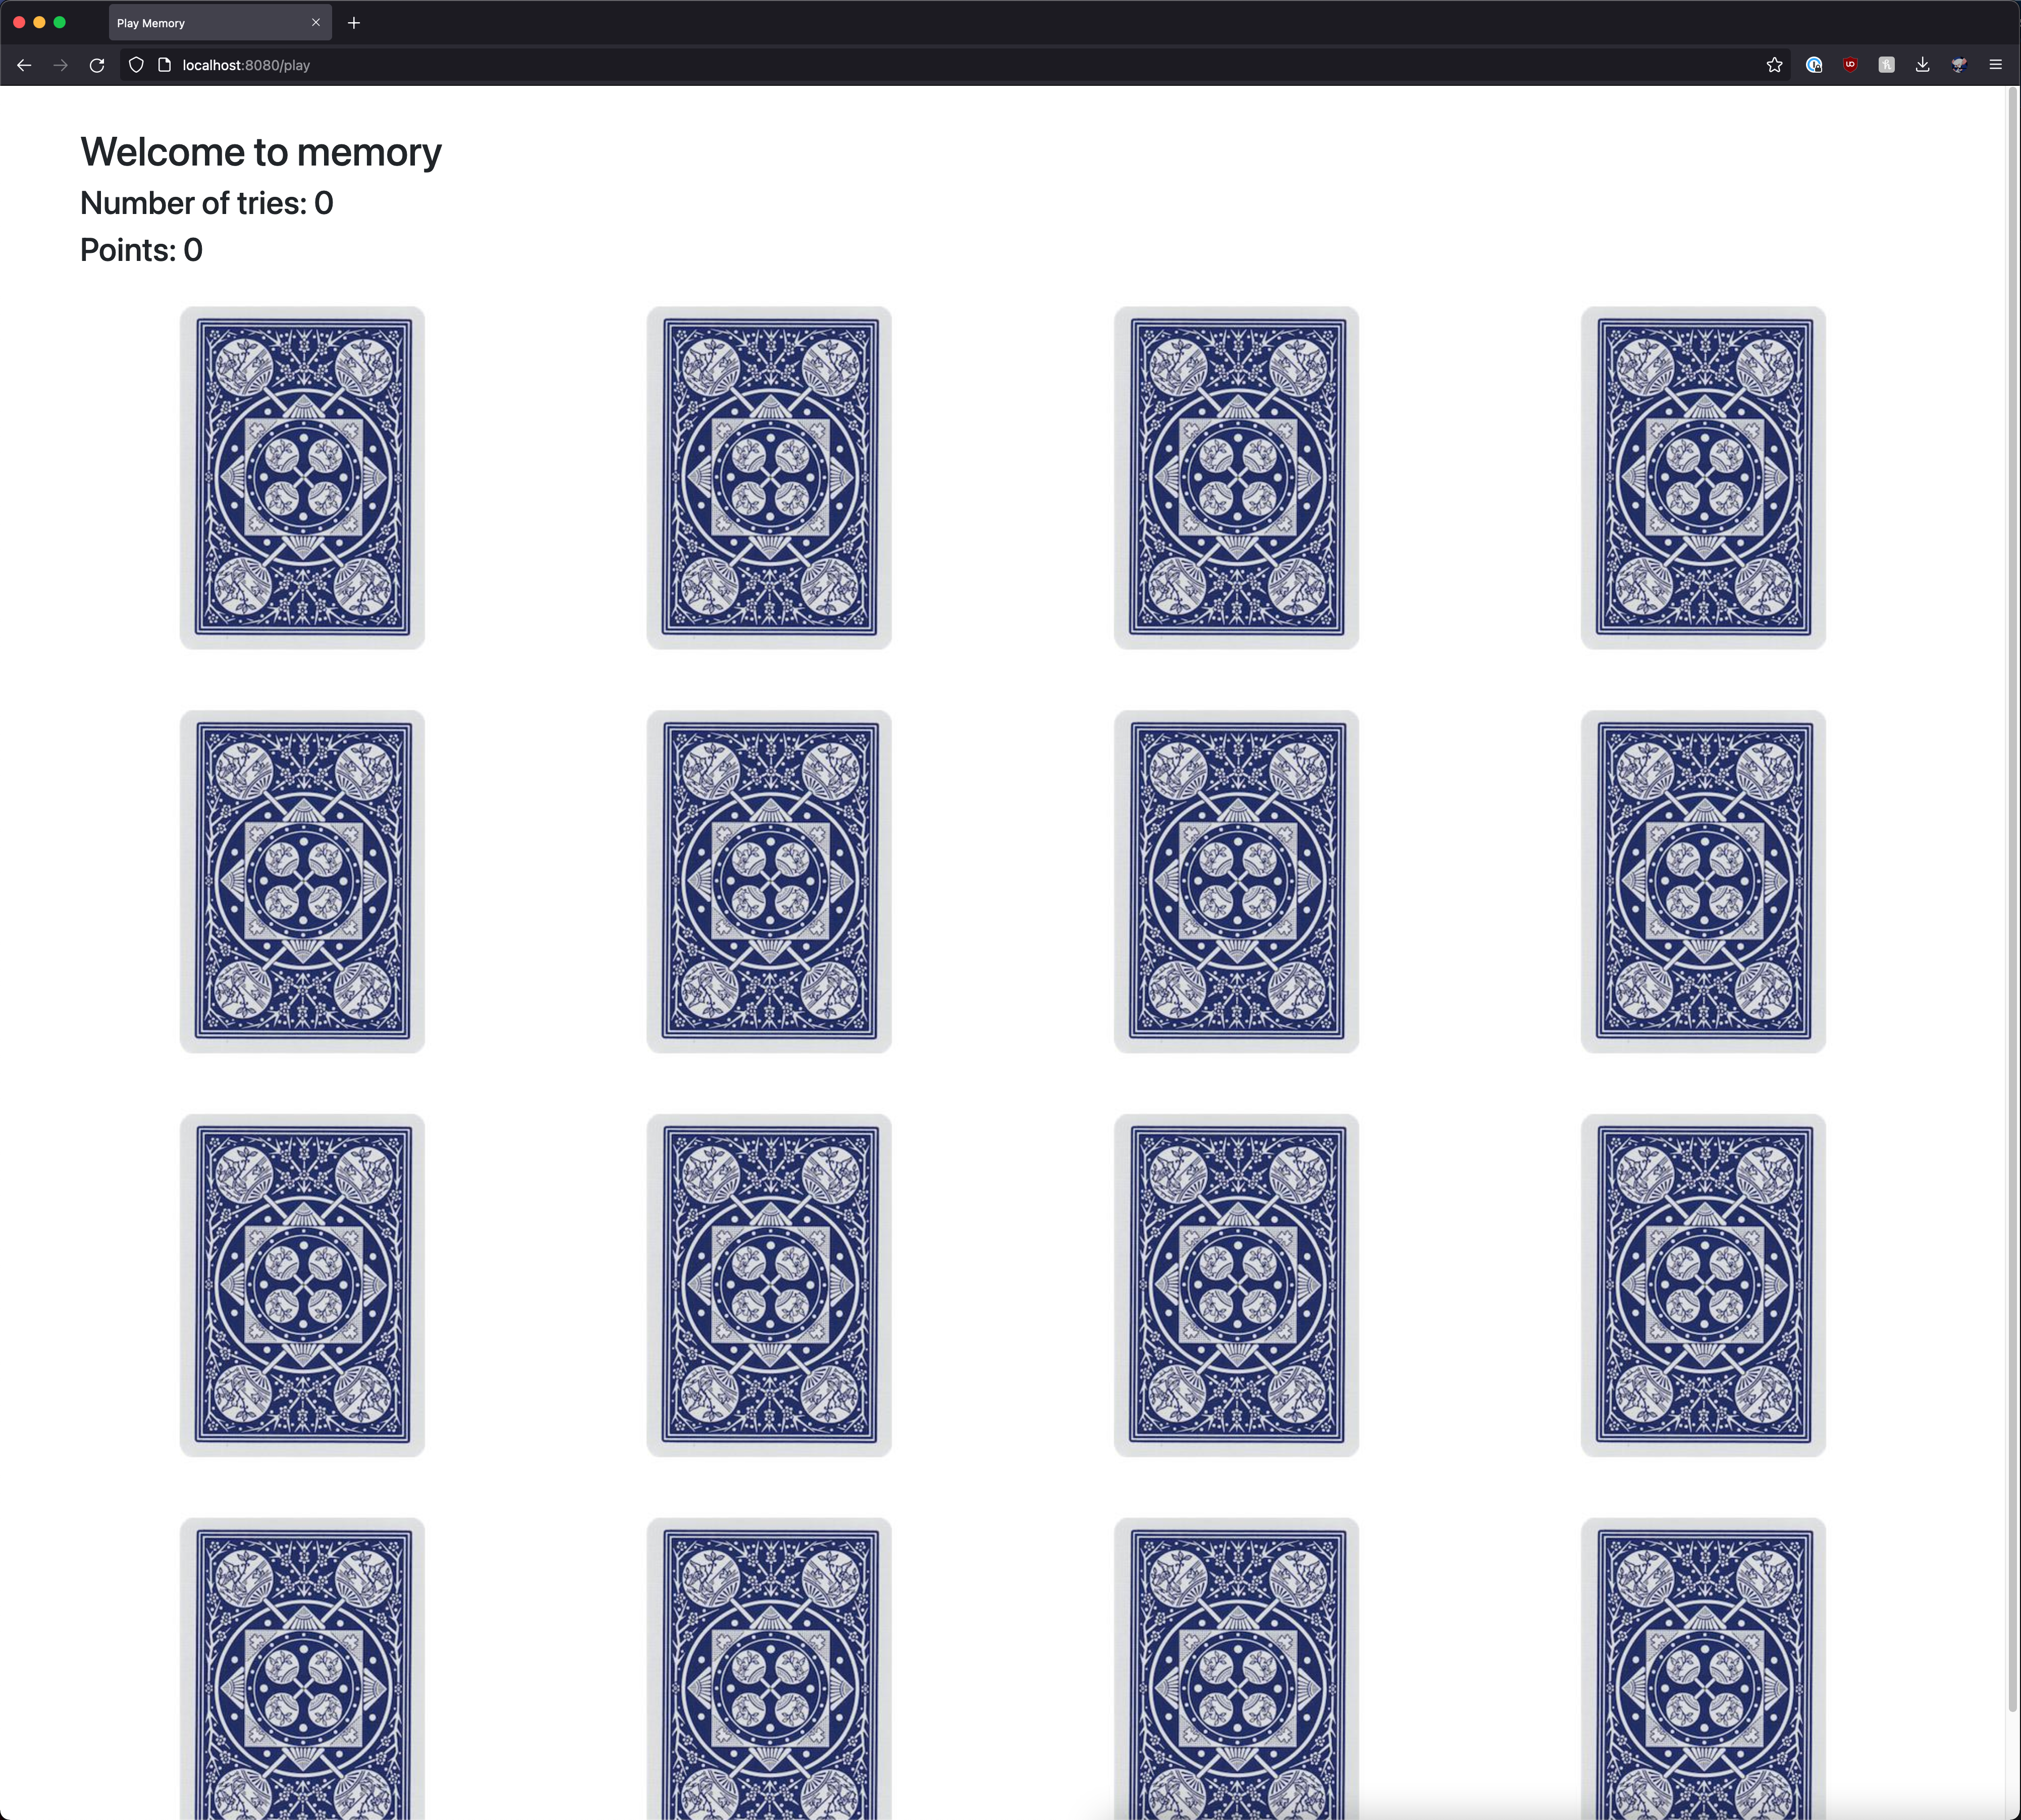
\includegraphics[scale=0.2]{images/03_impl/frontend/grid}
\caption{The Memory game grid}
\label{fig:03_impl_frontend_index_grid}
\end{figure}

\subsubsection{game.js}\label{subsubsec:03_impl_frontend_index}
% WHat
The \path{game.js} consists of a class called \texttt{Game}. This class is responsible to keep track of the state of the game.
% Events
The class gives the ability to register events. The events are: \texttt{onSelection}, \texttt{onSuccess}, \texttt{onFailure}, and \texttt{onGameEnded}. These events are triggered of the corresponding action happens.
% Selection
When the user makes a selection, the \texttt{onSelection} event is triggered. In addition, the \textit{Game} class keeps track of the first and second selection of a guess. Furthermore, it increases the number of tries.
% success
If the the user has made a second guess, and if the second guess is equal to the first guess, the \texttt{onSuccess} event is triggered. Additionally, the points are being updated as described in \Sec{subsec:02_design_frontend}.
% Failure
If the guess was wrong, the user was not able to find a pair, the \texttt{onFailure} event is triggered. Then, the points will be reduced.
% After selection
In both cases, success and failure, the first and second guess is set to \texttt{null} again.
%
When the number if tries is equal to 8, the game has ended and selections are disabled. Then, the \texttt{onGameEnded} event is triggered.

\subsubsection{memoryGame.js}\label{subsubsec:03_impl_frontend_memGame}
% What
the memoryGame.js handle the interaction between the UI (introduced in \Sec{subsubsec:03_impl_frontend_index}), and the \texttt{Game} class (introduced in \Sec{subsubsec:03_impl_frontend_index}).
% Game
After constructing the Game class, it registers all necessary events. This is shown in \Lst{lst:03_impl_frontend_memGame_events}.
% Listing
\begin{lstlisting}[label=lst:03_impl_frontend_memGame_events, caption=Register all events]
let game = new Game(8);
game.setEventListener("onSelection", onSelection);
game.setEventListener("onFailure", onFailure);
game.setEventListener("onSuccess", onSuccess);
game.setEventListener("onGameEnded", onGameEnded);
\end{lstlisting}


% DOM loaded
Furthermore, a function \texttt{startGame} exists, that is being called after the Document Object Model (DOM) is loaded. This is important to interact with UI. Then, it gets all card elements by using \texttt{document.getElementById} and adds an click event listener, that calls the \texttt{cardSelected} method of the Game class, for the event.

% If click is allowed
Click events are supposed to only work on cards, which presents the back (cards that have not been guessed already). Therefore, \texttt{memoryGame.js} keeps track of already guessed cards in the \texttt{alreadyGuessedElements} array. If the array contains the card element, the click listener will not be performed.
% first and second choice
Furthermore, the \texttt{memoryGame.js} saves the element of the first and the second guessed card, to flip those cards after a guess was incorrect, this is illustrated in \Fig{fig:03_impl_frontend_memGame_flipped}.
% Flipped figure
\begin{figure}[h]
\centering
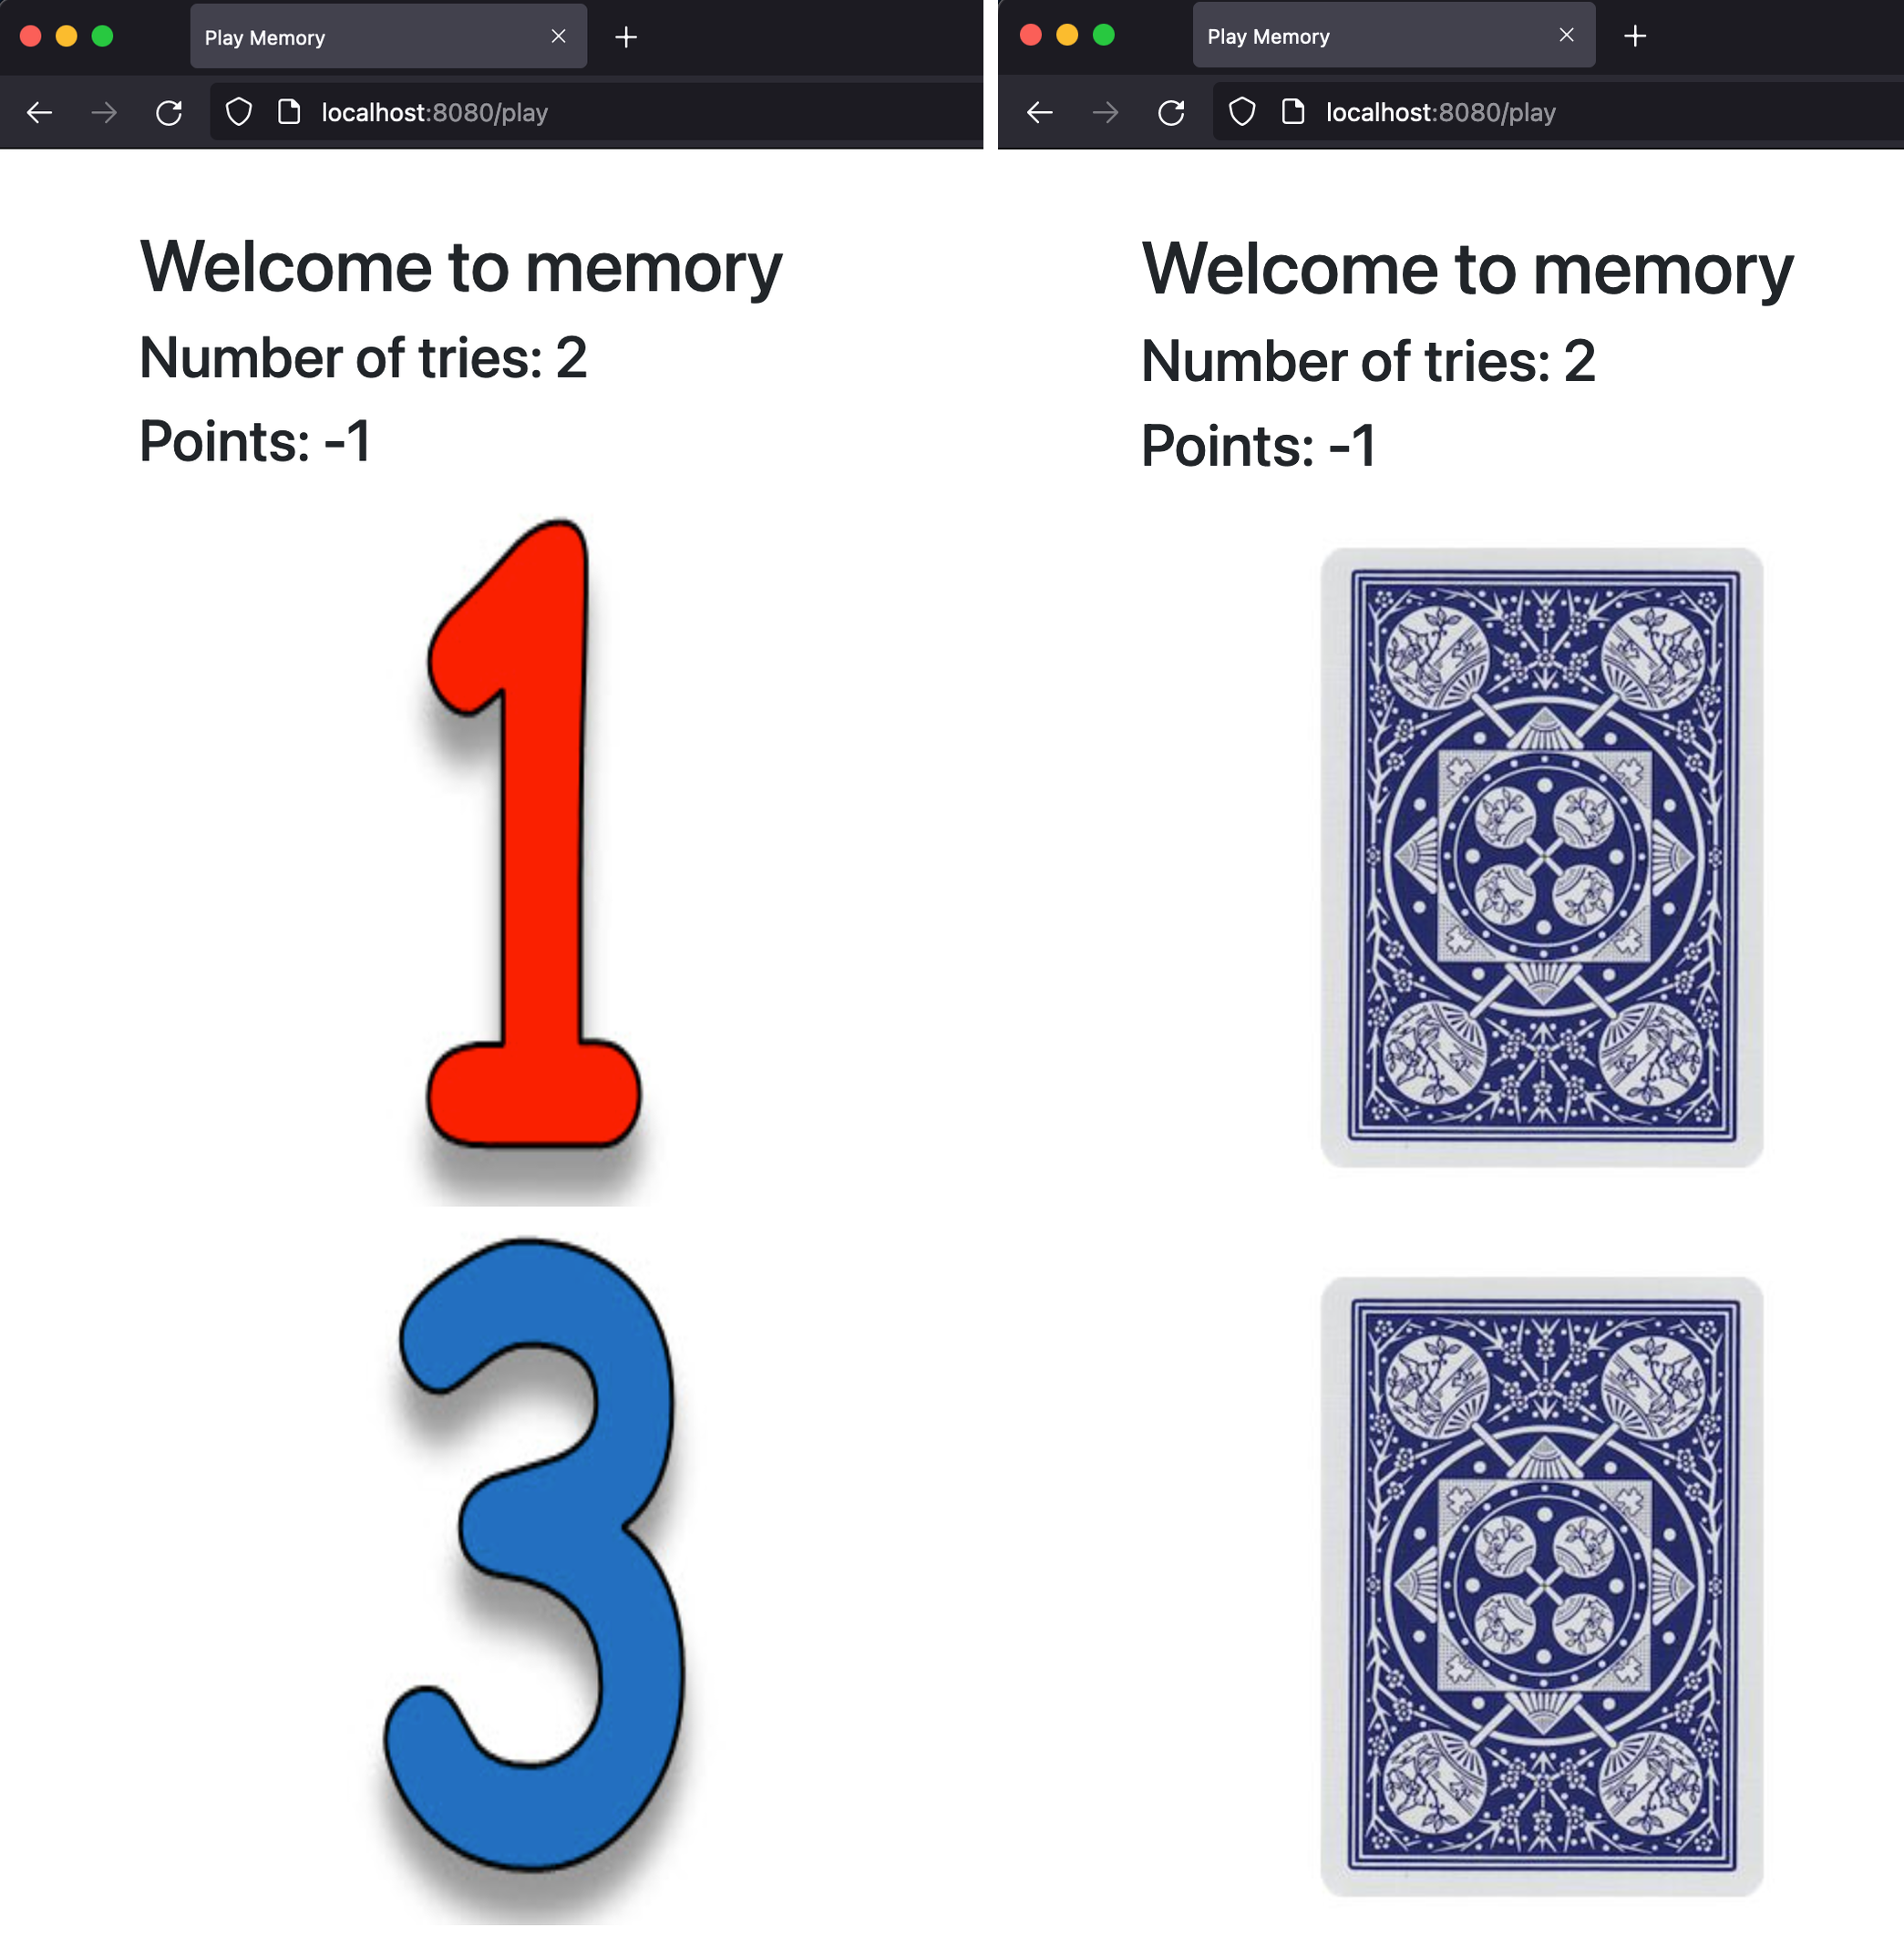
\includegraphics[scale=0.1]{images/03_impl/frontend/wrong-guess}
\caption{Flipped cards after a wrong guess}
\label{fig:03_impl_frontend_memGame_flipped}
\end{figure}


% On selection
If the Game class performs the \texttt{onSelection} event, \texttt{memoryGame.js} sends a \texttt{GET} request to the \textit{Memory-Grid-Servlet}. Then, the \textit{Memory-Grid-Servlet} sends back the value of the selected card, as described in \Sec{subsubsec:03_impl_backend_grid}. After that, the requested card value is forwarded to the \textit{Game} class via its \texttt{setSelection} method to check if a guess was correct and to update the points.
% Update UI
Additionally, the UI gets updated, by updating the card image element image \texttt{src} attribute to the selected value. Furthermore, the event updates the label that shows the number of tries.

% Success
As explained before, if a guess is correct, the \texttt{onSuccess} event is triggered. This event adds the elements of the guessed pair to the \texttt{alreadyGuessedElements} array to disable click events for this elements, and prevents the images to flip back (illustrated in \Fig{fig:03_impl_frontend_memGame_flippedCards}). Additionally, the points label gets updated.
% Success figure
\begin{figure}[h]
\centering
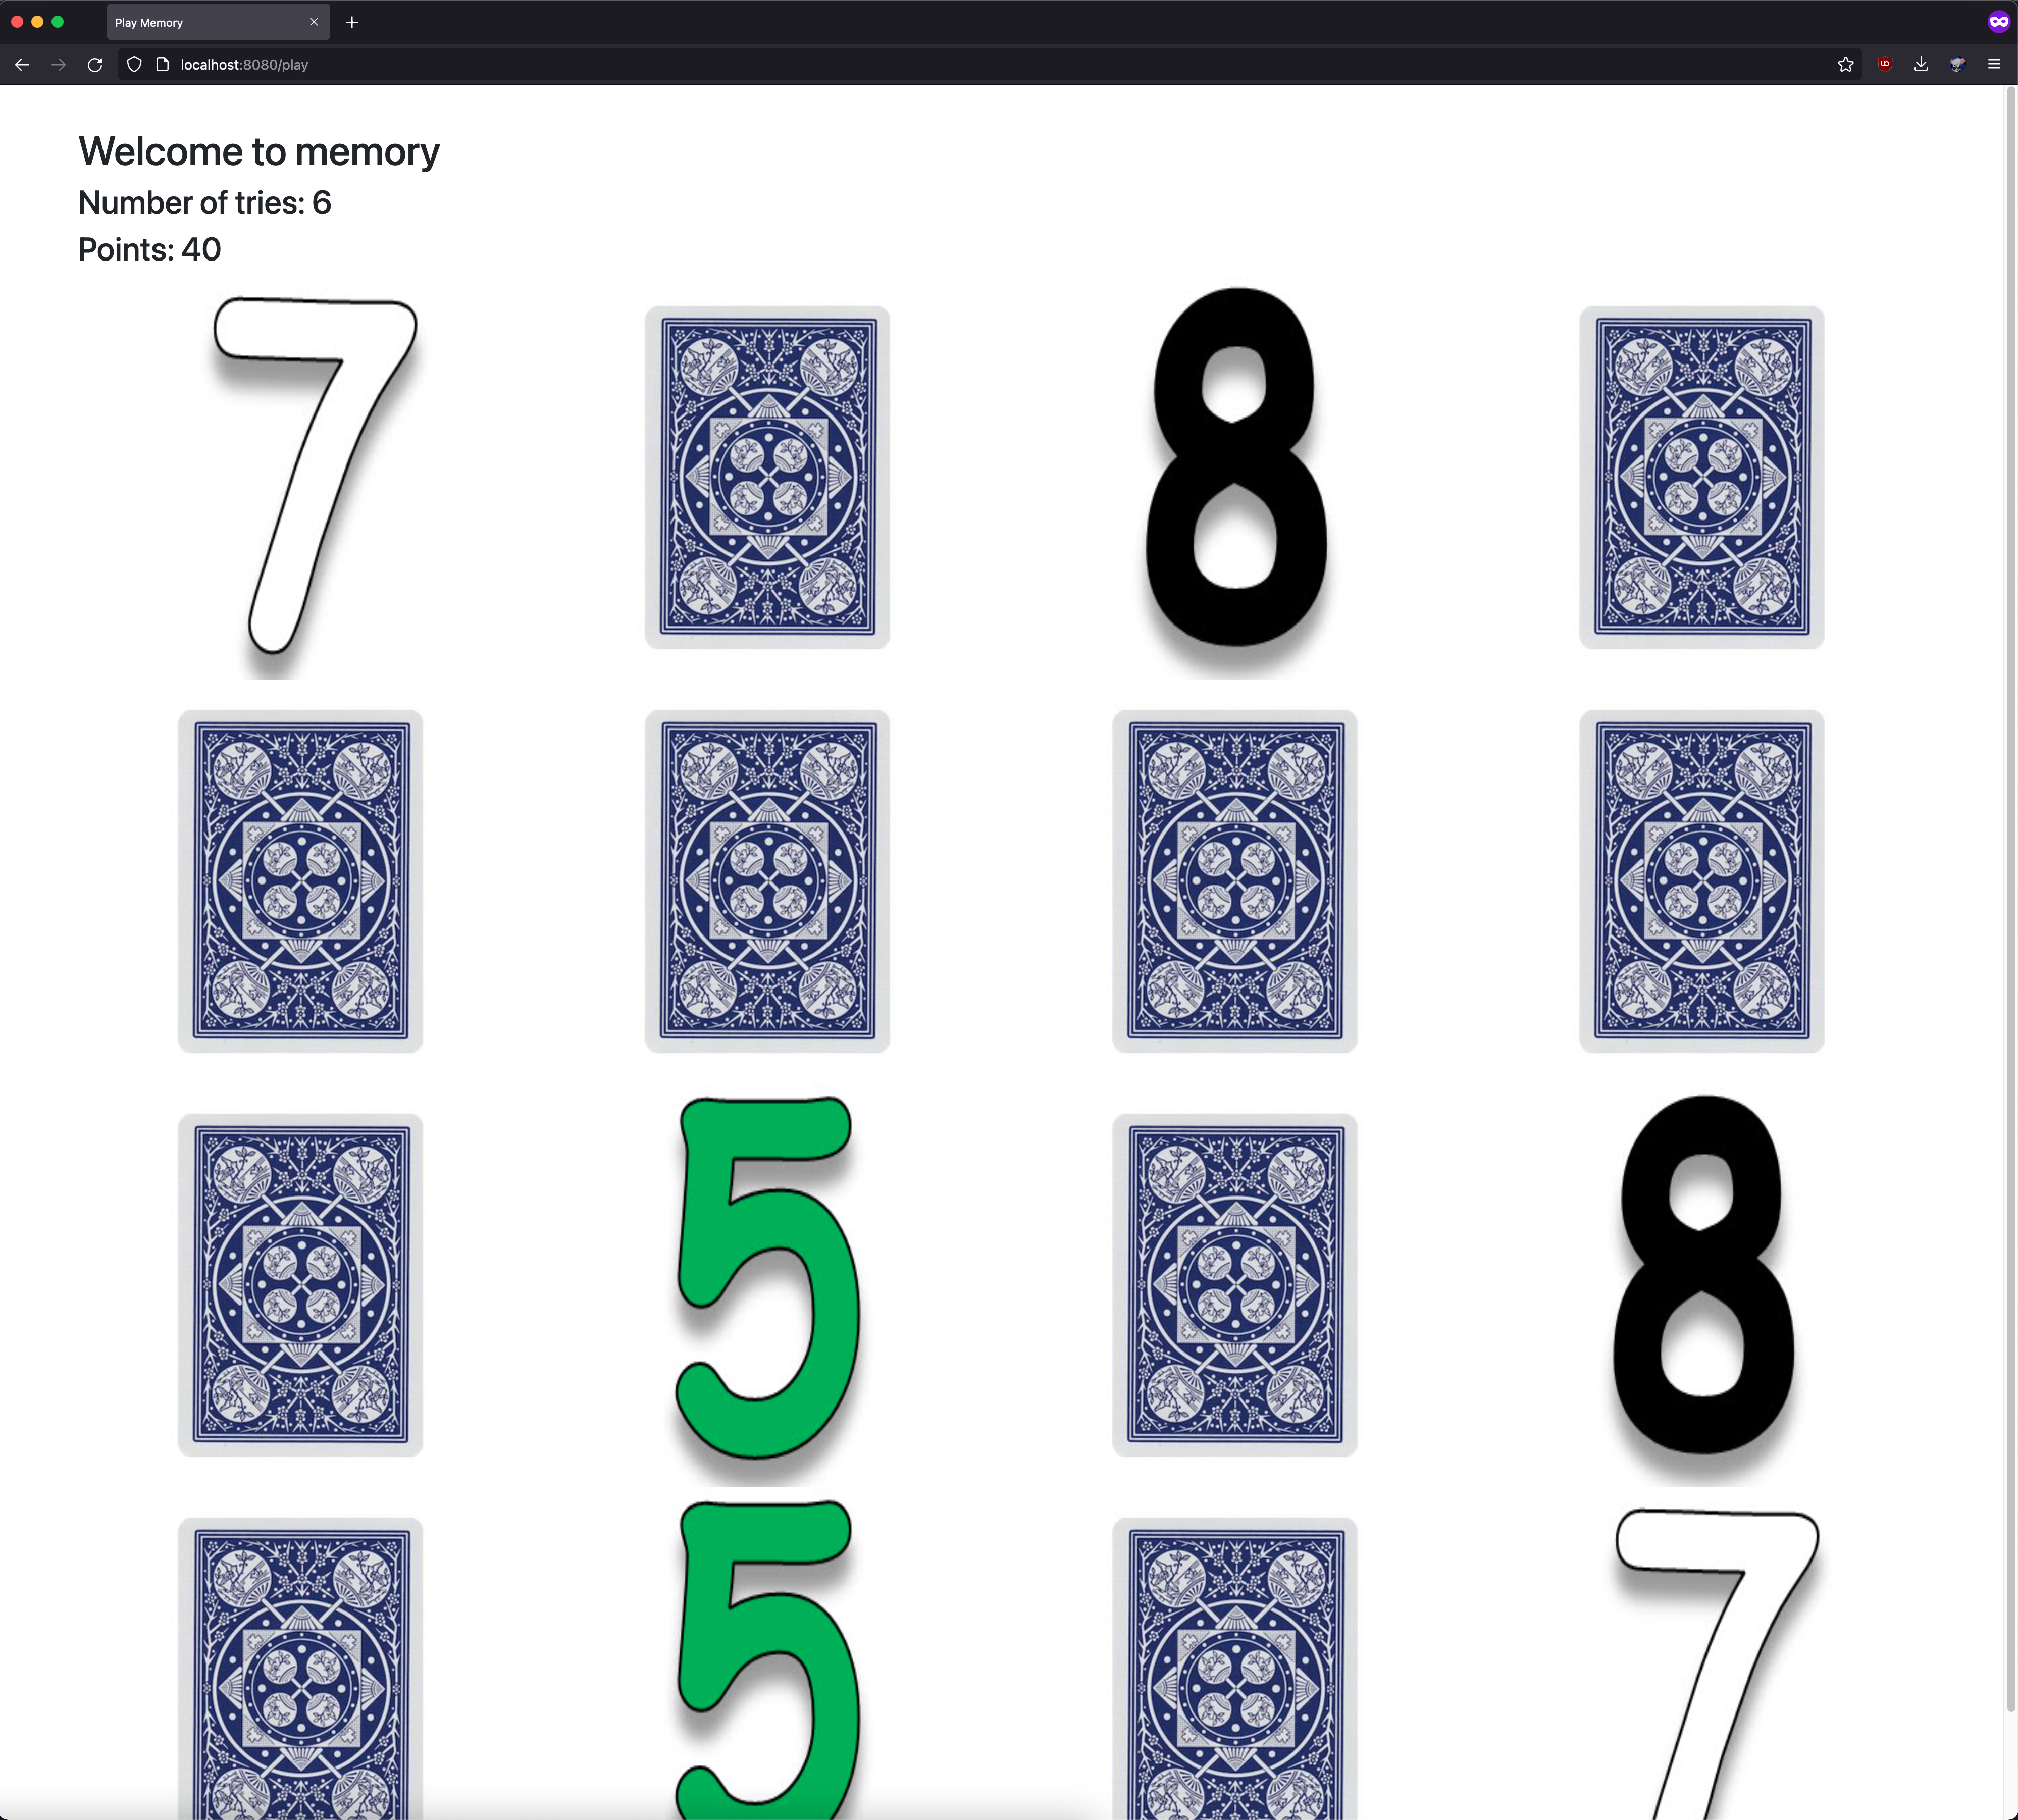
\includegraphics[scale=0.1]{images/03_impl/frontend/flipped-cards}
\caption{Three successful guesses}
\label{fig:03_impl_frontend_memGame_flippedCards}
\end{figure}
% Failure
If the guess is incorrect, the \texttt{onFailure} event is triggered. This events updates the points label, and flips back the cards after one second.
% Update labels figure
\begin{figure}[h]
\centering
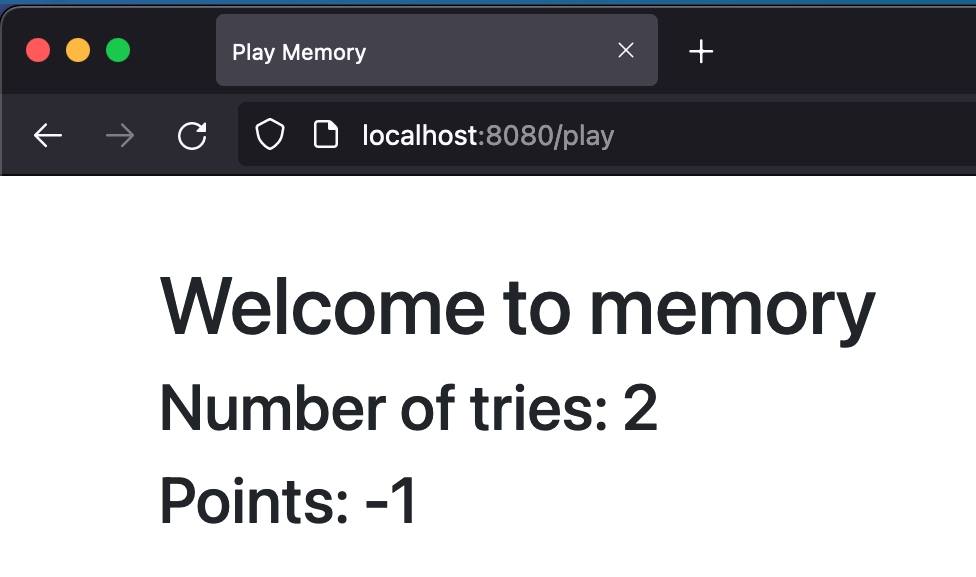
\includegraphics[scale=0.3]{images/03_impl/frontend/updated-labels}
\caption{Updated labels}
\label{fig:03_impl_frontend_memGame_updateLabels}
\end{figure}
% Explain
\Fig{fig:03_impl_frontend_memGame_updateLabels} shows the updated labels after \texttt{onSuccess} or \texttt{onFailure} was triggered.

\newpage
% onGameEnded
After 8 tries, the \texttt{onGameEnded} event is triggered by the Game class. Then, all cards are added to the \texttt{alreadyGuessedElements} array to disable click events. Additionally, a \texttt{POST} request is send to the \textit{Ranking-Servlet} given the achieved points in the game by the user. The \texttt{POST} request body has the content type \texttt{application/x-www-form-urlencoded}. If the response is successful, the \textit{Game Over} label is shown (shown in \Fig{fig:03_impl_frontend_memGame_gameOver}), and after 5 seconds, the user is redirected to the \textit{Ranking-Page}.
% Figure
\begin{figure}[h]
\centering
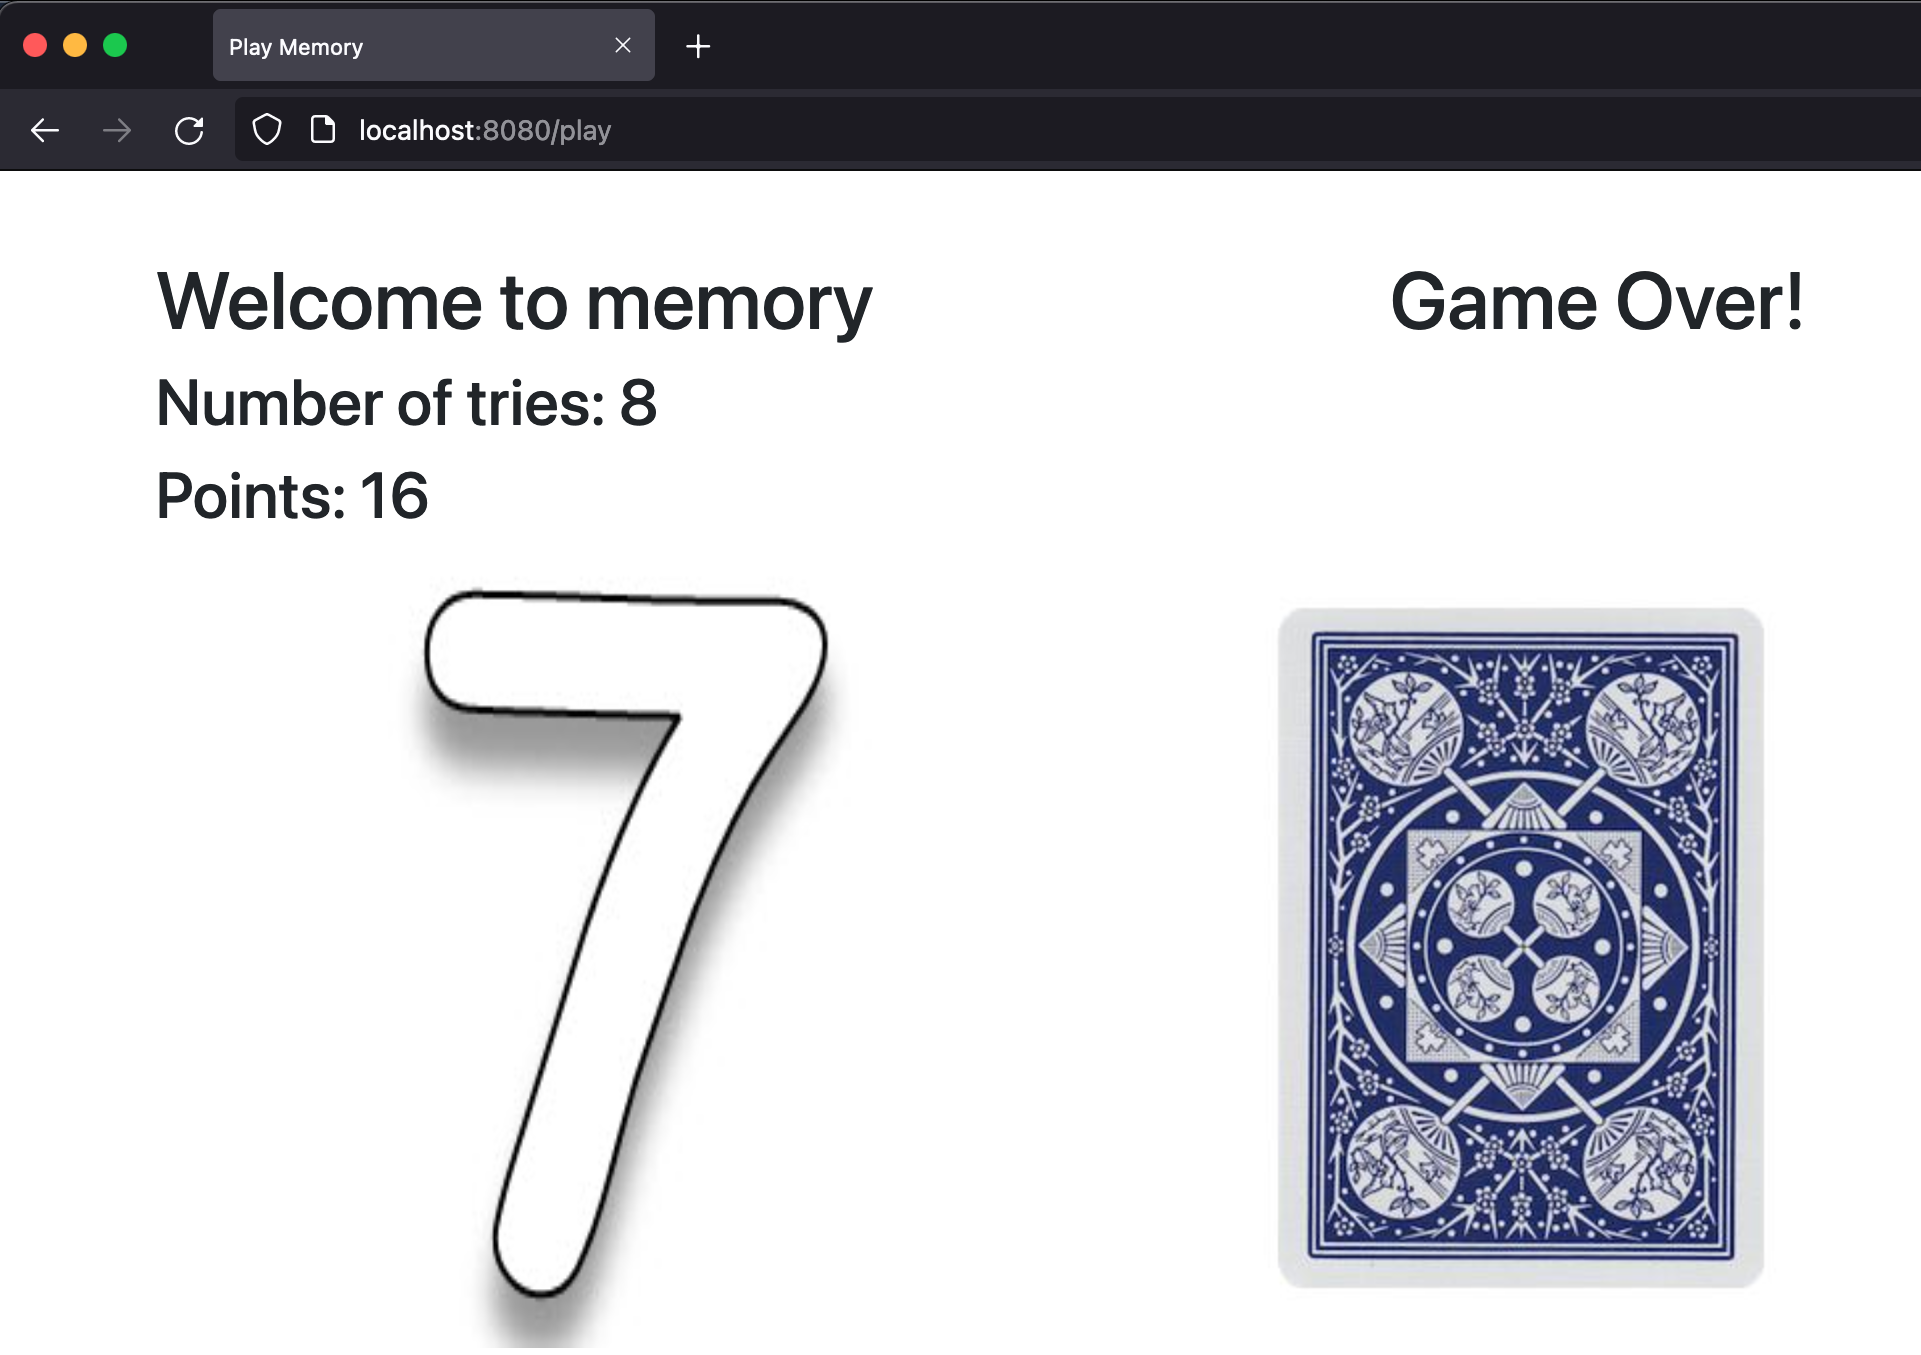
\includegraphics[scale=0.2]{images/03_impl/frontend/game-over}
\caption{The \textit{Game Over} label}
\label{fig:03_impl_frontend_memGame_gameOver}
\end{figure}
